\documentclass[12pt,a4]{article}
\usepackage[left=1.8cm,right=1.8cm,top=32mm,columnsep=20pt]{geometry}

\usepackage[utf8]{inputenc} %Formato de codificación
\usepackage[spanish, es-tabla, es-nodecimaldot]{babel}
\usepackage{amsmath} %paquete para escribir ecuaciones matemáticas
\usepackage{float} %Para posicionar figuras
\usepackage{graphicx} %Para poder poner figuras
\usepackage{hyperref} %Permite usar hipervínculos
\usepackage{multicol} %Para hacer doble columna
\usepackage[sorting=none]{biblatex} %Imports biblatex package. To cite use \cite{reference_label}
\usepackage{csquotes}

\title{Informe de Física: Encontrando el coeficiente de fricción dinámica}
\author{Francisco Carruthers, Facundo Firpo y Joel Jablonski\\ [2mm]
\small \texttt{\{fcarruthers, ffirpo, jjablonski\}@udesa.edu.ar}\\
\small Grupo 4\\
\small Fisica I, tutorial Vinograd}
\date{2do Semestre 2024}


\begin{document}

\maketitle

\begin{abstract}
    Utilizando un carrito, una soga y una polea, se busca encontrar el coeficiente de fricción dinámica entre el carrito y la superficie. Para ello, se mide la aceleración del carrito con distintas masas y se calcula el coeficiente de fricción dinámica. También, utilizamos varias superficies para ver cómo afecta el coeficiente de fricción.
\end{abstract}

\section{Introducción}

(Descripción del experimento)

(Desarrollo de Newton y Vinculos del problema)

\begin{table}
    \centering
    \begin{tabular}{|c|c|}
        \hline
        \textbf{Objeto} & \textbf{Masa(g)} \\
        \hline
        Pesa dorada & 72 +- 1 \\
        Pesa plateada & 23 +- 1 \\
        Pesa madera & 6 +- 1 \\
        Trineo & 109 +- 1 \\
        Metro & 134 +- 1 \\
        \hline
    \end{tabular}
    \caption{Mediciones de masa}
    \label{tab:mediciones}
\end{table}

\newpage
\section{Calibración}

Utilizamos un sistema de referencia para calibrar el sistema.

\begin{figure}[H]
    \centering
    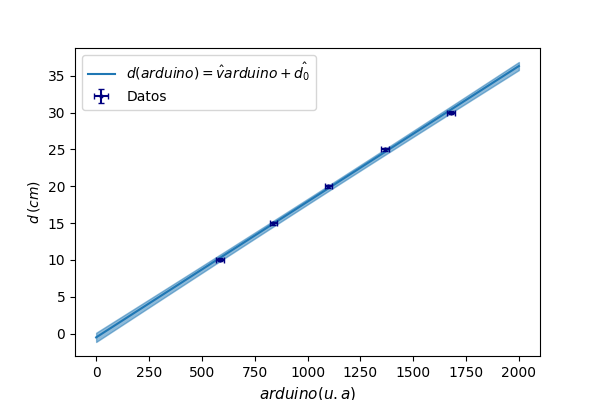
\includegraphics[width=0.9\linewidth]{Calibracion.png}
    \caption{Calibración del sistema}
    \label{fig:calibracion}
\end{figure}

Pendiente: 0.0184 ± 0.0005 \\

Ordenada al origen: -0.508 ± 0.532 \\

Distancia para 600: 10.54 ± 0.44 cm \\

\section{Resultados}

\subsection{Papel y Papel}

\subsubsection{$M = 243 \pm 1, m = 72 \pm 1$}

En un primer caso pusimos el metro en el carrito y la pesa dorada en el extremo de la soga.

Usando los datos del sensor Arduino, podemos calcular la distancia recorrida en función del tiempo.

\begin{figure}[H]
    \centering
    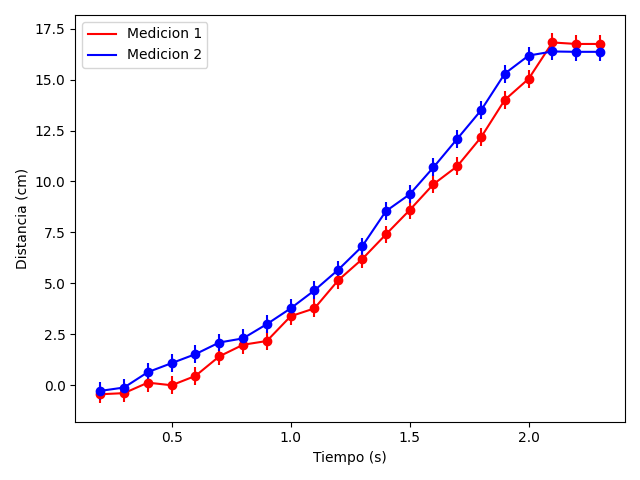
\includegraphics[width=0.9\linewidth]{TiempoVsDistanciaPapelPapelM_O.png}
    \caption{Papel y Papel, m = Metro y M = Pesa dorada}
    \label{fig:PyPM_O}
\end{figure}

Usamos un ajuste cuadrático para encontrar la aceleración.

\begin{figure}[H]
    \centering
    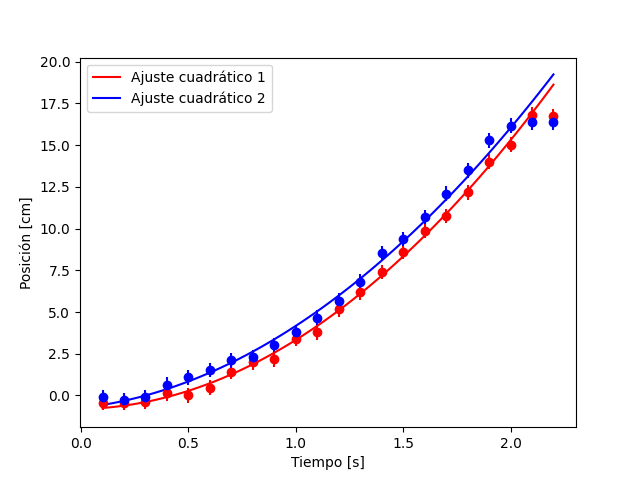
\includegraphics[width=0.9\linewidth]{ajuste2_PapelPapelM_O.png}
    \caption{Ajuste cuadratico}
    \label{fig:a2PPM_O}
\end{figure}

Con $Pos_1(t) = (3.91 \pm 0.33) t^2 + (0.23 \pm 0.78) t + (-0.81 \pm 0.40)$

\newpage
Graficamos las aceleraciones en función de las masas.

\begin{figure}[H]
    \centering
    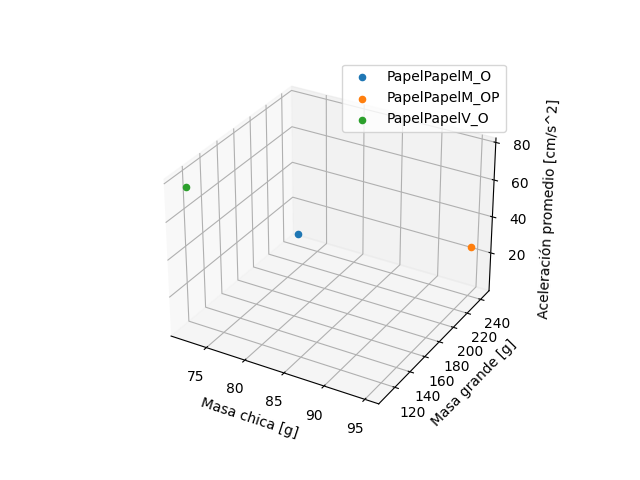
\includegraphics[width=0.9\linewidth]{scatter_aceleraciones.png}
    \caption{Aceleraciones vs m y M}
    \label{fig:aPPM_O}
\end{figure}

(No se ve del todo bien, probablemente haya que cambiar la manera de graficar) \\

Utilizando estas aceleraciones, reemplazamos en la ecuacion para el $\mu_d$ y encontramos que $\mu_d$ de rozamiento entre papel y papel es 21.22 N. (falta la incerteza)

\end{document}